%	The main skeletal structure
	\documentclass[crop,tikz,convert={outext=.svg,command=\unexpanded{/opt/homebrew/bin/pdf2svg \infile\space\outfile}},multi=false]{standalone}
%	\def\pgfsysdriver{pgfsys-tex4ht.def}
%	\documentclass[twocolumn]{report}
	\usepackage{setspace}
	\usepackage{graphicx}
		\DeclareGraphicsExtensions{.pdf,.png,.eps,.ps}
	\usepackage{subcaption}
	\usepackage{lscape}
	\usepackage{pifont}
%	\usepackage{bbding}
	\usepackage{multirow}
	\usepackage{longtable}
	\usepackage[version=4]{mhchem}
	\usepackage{xfrac}
	\usepackage{color}
	\usepackage[colorlinks=true]{hyperref}
	\usepackage{gensymb}
	\usepackage{multicol}
		\setlength{\columnseprule}{0.4pt}
		\setlength{\columnsep}{5mm}
\makeatletter 
\newcounter{reaction} 
%%% >> for article << 
%\renewcommand\thereaction{C\,\arabic{reaction}} 
%%% << for article << 
%%% >> for report and book >> 
\renewcommand\thereaction{C\,\thechapter.\arabic{reaction}} 
\@addtoreset{reaction}{chapter} 
%%% << for report and book << 
\newcommand\reactiontag{\refstepcounter{reaction}\tag{\thereaction}} 
\newcommand\reaction@[2][]{\begin{equation}\ce{#2}% 
\ifx\@empty#1\@empty\else\label{#1}\fi% 
\reactiontag\end{equation}} 
\newcommand\reaction@nonumber[1]{\begin{equation*}\ce{#1}% 
\end{equation*}} 
\newcommand\reaction{\@ifstar{\reaction@nonumber}{\reaction@}} 
\makeatother 


	\usepackage[a4paper]{geometry}
	\usepackage{fullpage}
	\usepackage{fancyhdr}
%		\pagestyle{fancy}
%		\lhead{}
%		\chead{}
%		\rhead{\slshape \rightmark}
%		\fancyhead[LO,RE]{\slshape \leftmark} 
%		\fancyfoot[R]{\thepage} 
%	\renewcommand{\headrulewidth}{0.4pt} 
%	\renewcommand{\footrulewidth}{0.4pt} 
	\usepackage{cite}
	
%	\onehalfspacing
	\renewcommand{\baselinestretch}{1.5}
	
%	Footnote symbols
	\renewcommand{\thefootnote}{\fnsymbol{footnote}}

% Defining the chapter abstract area
%	\newenvironment{abstract}{\rightskip1in}{}

% Allow standard state notation
	\usepackage[varioref=false]{chemstyle}

% Allow for numbered examples
%	\usepackage{theorem,lipsum}
%	\theorembodyfont{\upshape}
%	\newtheorem{example}{Example}[chapter]
%	\newtheorem{question}{Question}[chapter]
%	\newtheorem{exercise}{Exercise}[chapter]
%	\newtheorem{concept}{Key Concept}[chapter]
%%%%%\begin{example}
%%%%%This is an example?
%%%%%\end{example}
%%%%%
%%%%%\begin{question}
%%%%%This is a quesiton?
%%%%%\end{question}

%%%%%FONT STUFF

%\usepackage[defaultfam,extralight,tabular,lining]{montserrat} %% Option 'defaultfam'
%%% only if the base font of the document is to be sans serif
%\usepackage[T1]{fontenc}
%\renewcommand*\oldstylenums[1]{{\fontfamily{Montserrat-TOsF}\selectfont #1}}

\usepackage{arev}
\usepackage[T1]{fontenc}
\usepackage{soul}

%%%%%TIKZ stuff
	\usepackage{tikz}
	\usepackage{pgfplots}
	\usetikzlibrary{decorations.pathmorphing,patterns,arrows,shapes.arrows}
	\usepgfplotslibrary{fillbetween}
	\tikzset{every picture/.style=remember picture}
		\newcommand{\mathnode}[1]{%
		\mathord{\tikz[baseline=(#1.base), inner sep = 0pt]{\node (#1) {$#1$};}}}

%%%%%% Grey stuff
%Need to define a shitload of greys...
\definecolor{gray1}{RGB}{240,240,240}
\definecolor{gray2}{RGB}{225,225,225}
\definecolor{gray3}{RGB}{210,210,210}
\definecolor{gray4}{RGB}{200,200,200}
\definecolor{gray5}{RGB}{180,180,180}


\begin{document}

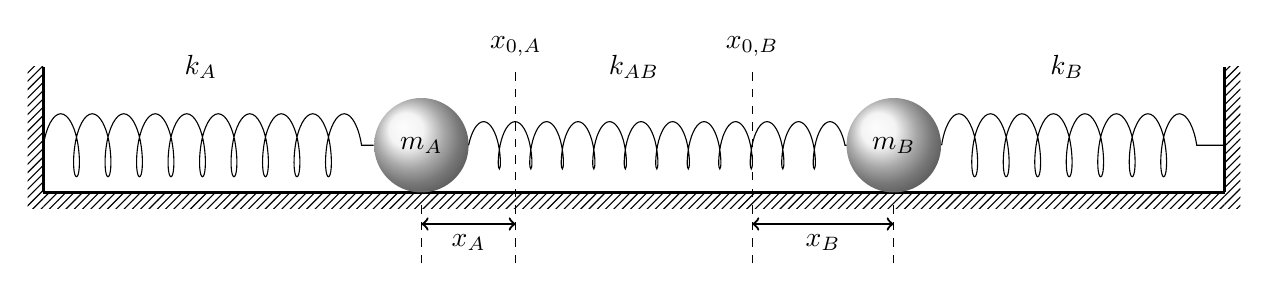
\begin{tikzpicture}[scale=1]

\def\xa{4.8}
\def\xb{10.8}

\fill [pattern = north east lines] (-0.2,-0.8) rectangle (0,1);
\fill [pattern = north east lines] (0,-0.8) rectangle (15,-0.6);
\fill [pattern = north east lines] (15,-0.8) rectangle (15.2,1);


\draw[thick] (0,-0.6) -- (0,1);
\draw[thick] (0,-0.6) -- (15,-0.6);
\draw[thick] (15,-0.6) -- (15,1);

\node[] (a) at (0,0) {};
\node[circle,ball color=gray1,inner sep=0mm,minimum size=1.2cm] (b) at (\xa,0) {$m_A$};

\node[] (c) at (15,0) {};
\node[circle,ball color=gray1,inner sep=0mm,minimum size=1.2cm] (d) at (\xb,0) {$m_B$};

\draw[decoration={aspect=0.3, segment length=4mm, amplitude=4mm,coil},decorate] (0,0) -- (b); 
\node[] at (2,1) {$k_A$};
\node[] at (13,1) {$k_B$};
\node[] at (7.5,1) {$k_{AB}$};

\draw[decoration={aspect=0.3, segment length=4mm, amplitude=4mm,coil},decorate] (d) --(15,0) ; 

\draw[decoration={aspect=0.3, segment length=4mm, amplitude=3mm,coil},decorate] (\xa+0.6,0) --(\xb-0.6,0) ; 

% \draw[|-|,thick](0,-1)-- node[below] {$x_\textrm{0}$} (6,-1);
\draw[,dashed](6,-1.5)-- (6,1) node[above]{$x_{0,A}$} ;
\draw[,dashed](9,-1.5)-- (9,1) node[above]{$x_{0,B}$} ;

\draw[,dashed](\xa,-1.5)-- node[below] {} (\xa,-0.75);
\draw[<->,thick](\xa,-1)-- node[below] {$x_A$} (6,-1);

\draw[,dashed](\xb,-1.5)-- node[below] {} (\xb,-0.75);
\draw[<->,thick](9,-1)-- node[below] {$x_B$} (\xb,-1);


%
%\node[circle,ball color=gray,inner sep=5mm] (a) at (0,-2.5) {};
%\node[circle,ball color=gray,inner sep=5mm] (b) at (6,-2.5) {};
%\draw[decoration={aspect=0.2, segment length=3.04mm, amplitude=4mm,coil},decorate] (a) -- (b); 
%\draw[|-|,thick](0,-3.5)-- node[below] {$r_\textrm{0}$} (4.5,-3.5);
%\draw[<->|,thick](4.5,-3.5)-- node[below] {$R$} (6,-3.5);
%\draw[|<->|,thick](0,-4.5)-- node[below] {$r$} (6,-4.5);
\end{tikzpicture}

\end{document}

% Use the following to include the graphics in the chapter
%
%
%\begin{figure}[htbp]
%\begin{center}
%\includegraphics[scale=0.5]{images/fig-ch7_harmonicoscill0.pdf}
%\caption[Caption for list of figures]{Full caption to appear beside the image}
%\label{fig:label}
%\end{center}
%\end{figure}
 